\section{Deep Q-Learning}
\subsection{Introduction}

Part 1 of this assignment requires you to implement and evaluate Q-learning for playing Atari games. The Q-learning algorithm was covered in lecture, and you will be provided with starter code. This assignment will be faster to run on a GPU, though it is possible to complete on a CPU as well. Note that we use convolutional neural network architectures in this assignment. Therefore, we recommend using the Colab option if you do not have a GPU available to you. Please start early!

% The questions will require you to perform multiple runs of Q-learning, each of which can take quite a long time. Furthermore, depending on your implementation, you may find it necessary to tweak some of the parameters, such as learning rates or exploration schedules, which can also be very time consuming. The actual coding for this assignment will involve about 50 lines of code, but the evaluation will take longer than in the previous two assignments.

\subsection{File overview}
The starter code for this assignment can be found at

\begin{centering}
\url{https://github.com/berkeleydeeprlcourse/homework_fall2023/tree/main/hw3} \\
\end{centering}
\vspace{.35cm}

You will implement a DQN agent in \verb|cs285/agents/dqn_agent.py| and \verb|cs285/scripts/run_hw3_dqn.py|. In addition to those two files, you should start by reading the following files thoroughly:
\begin{itemize}
    \item \verb|cs285/env_configs/dqn_basic.py|: builds networks and generates configuration for the basic DQN problems (cartpole, lunar lander).
    \item \verb|cs285/env_configs/dqn_atari.py|: builds networks and generates configuration for the Atari DQN problems.
    \item \verb|cs285/infrastructure/replay_buffer.py|: implementation of replay buffer. You don't need to know how the memory efficient replay buffer works, but you should try to understand what each method does (particularly the difference between \verb|insert|, which is called after a frame, and \verb|on_reset|, which inserts the first observation from a trajectory) and how it differs from the regular replay buffer.
    \item \verb|cs285/infrastructure/atari_wrappers.py|: contains some wrappers specific to the Atari environments. These wrappers can be key to getting challenging Atari environments to work!
\end{itemize}

There are two new package requirements (\texttt{gym[atari]} and \texttt{pip install gym[accept-rom-license]}) beyond what was used in the first two assignments; make sure to install these with \texttt{pip install -r requirements.txt} if you're re-using your Python environment from last assignment.

\subsection{Implementation}

The first phase of the assignment is to implement a working version of Q-learning, with some extra bells and whistles like double DQN. Our code will work with both state-based environments, where our input is a low-dimensional list of numbers (like Cartpole), but we'll also support learning directly from pixels!

In addition to the double $Q$-learning trick (which you'll implement later), we have a few other tricks implemented to stabilize performance. You don't have to do anything to enable these, but you should look at the implementations and think about why they work.
\begin{itemize}
    \item \textbf{Exploration scheduling for $\epsilon$-greedy actor.} This starts $\epsilon$ at a high value, close to random sampling, and decays it to a small value during training.
    \item \textbf{Learning rate scsheduling.} Decay the learning rate from a high initial value to a lower value at the end of training.
    \item \textbf{Gradient clipping.} If the gradient norm is larger than a threshold, scale the gradients down so that the norm is equal to the threshold.
    \item \textbf{Atari wrappers.}
    \begin{itemize}
        \item \textbf{Frame-skip.} Keep the same constant action for 4 steps.
        \item \textbf{Frame-stack.} Stack the last 4 frames to use as the input.
        \item \textbf{Grayscale.} Use grayscale images.
        % \item \textbf{Fire-reset.} Some Atari games require pressing the ``fire'' button to start the game. In these environments, do this automatically.
    \end{itemize}
\end{itemize}

\subsection{Basic Q-Learning}

Implement the basic DQN algorithm. You'll implement an update for the $Q$-network, a target network, and 

\textbf{What you'll need to do}:
\begin{itemize}
    \item Implement a DQN critic update in \verb|update_critic| by filling in the unimplemented sections (marked with TODO(student)).
    \item Implement $\epsilon$-greedy sampling in \verb|get_action|
    \item Implement the TODOs in \verb|run_hw3_dqn.py|.

    \textbf{Hint:} A trajectory can end (\verb|done=True|) in two ways: the actual end of the trajectory (usually triggered by catastrophic failure, like crashing), or \textit{truncation}, where the trajectory doesn't actually end but we stop simulation for some reason (commonly, we truncate trajectories at some maximum episode length). In this latter case, you should still reset the environment, but the \verb|done| flag for TD-updates (stored in the replay buffer) should be false.
    \item Call all of the required updates, and update the target critic if necessary, in \verb|update|.
\end{itemize}

\textbf{Testing this section}:
\begin{itemize}
    \item Debug your DQN implementation on \verb|CartPole-v1| with \verb|experiments/dqn/cartpole.yaml|. It should reach reward of nearly 500 within a few thousand steps.
\end{itemize}

\textbf{Deliverables}:
\begin{itemize}
    \item Submit your logs of \verb|CartPole-v1|, and a plot with environment steps on the $x$-axis and eval return on the $y$-axis.
    \item Run DQN with three different seeds on \verb|LunarLander-v2|:
\begin{lstlisting}[language=bash,breaklines=true]
  python cs285/scripts/run_hw3_dqn.py -cfg experiments/dqn/lunarlander.yaml --seed 1
  python cs285/scripts/run_hw3_dqn.py -cfg experiments/dqn/lunarlander.yaml --seed 2
  python cs285/scripts/run_hw3_dqn.py -cfg experiments/dqn/lunarlander.yaml --seed 3
\end{lstlisting}
\textbf{Your code may not reach high return (200) on Lunar Lander yet; this is okay!} Your returns may go up for a while and then collapse in some or all of the seeds.
    \item Run DQN on \verb|CartPole-v1|, but change the \verb|learning rate| to 0.05 (you can change this in the YAML config file). What happens to (a) the predicted $Q$-values, and (b) the critic error? Can you relate this to any topics from class or the analysis section of this homework?
\end{itemize}

\textbf{Result:}
\begin{figure}[H]
    \centering
    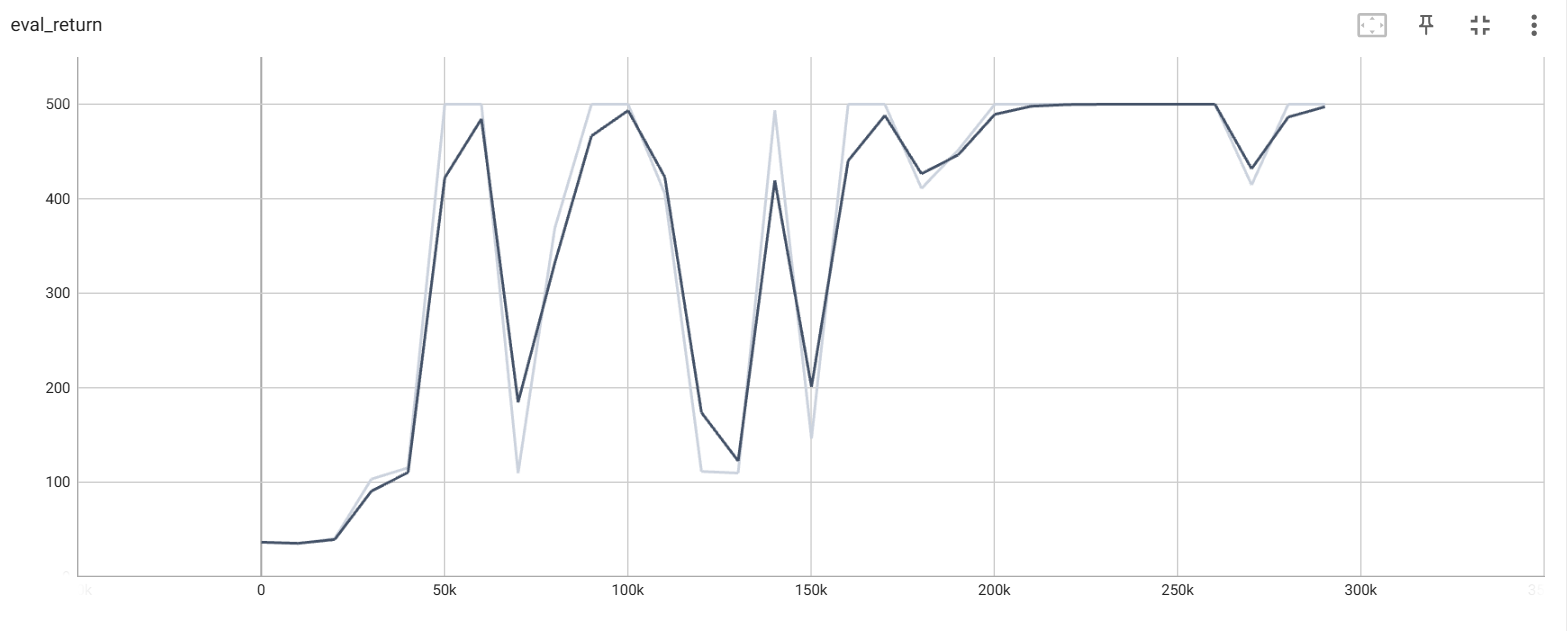
\includegraphics[width=0.8\textwidth]{imgs/dqn/cartpole.png}
    \caption{CartPole DQN results}
    \label{fig:cartpole_dqn}
\end{figure}

\begin{figure}[H]
    \centering
    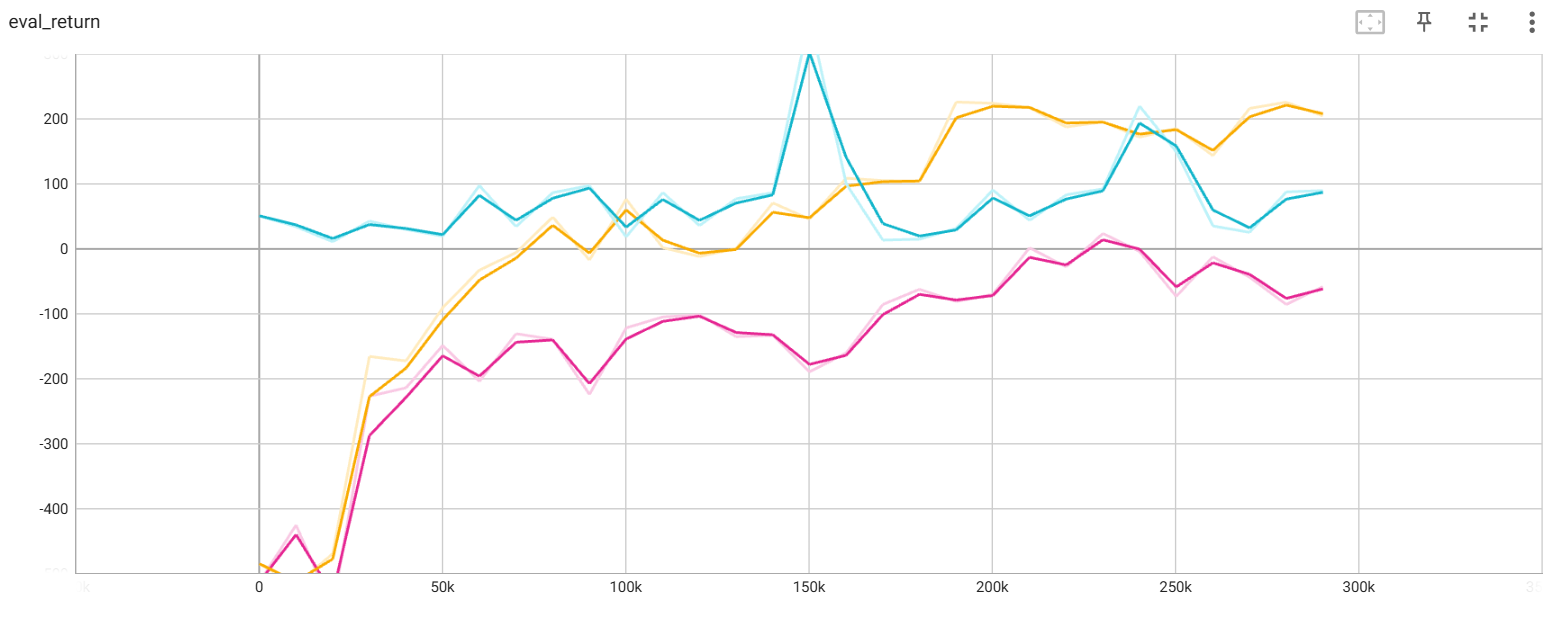
\includegraphics[width=0.8\textwidth]{imgs/dqn/lunarlander.png}
    \caption{Lunar Lander DQN results}
    \label{fig:lunarlander}
\end{figure}



\subsection{Double Q-Learning}
Let's try to stabilize learning. The double-Q trick avoids overestimation bias in the critic update by using two different networks to \textit{select} the next action $a'$ and to \textit{estimate} its value:
\[a' = \textrm{arg}\max_{a'} Q_{\phi}(s', a')\]
\[Q_{\textrm{target}} = r + \gamma(1-d_t) Q_{\phi'}(s', a').\]
In our case, we'll keep using the target network $Q_{\phi'}$ to estimate the action's value, but we'll select the action using $Q_{\phi}$ (the online $Q$ network).

Implement this functionality in \verb|dqn_agent.py|.

\textbf{Deliverables}:
\begin{itemize}
    \item Run three more seeds of the lunar lander problem:
\begin{lstlisting}[language=bash,breaklines=true]
  python cs285/scripts/run_hw3_dqn.py -cfg experiments/dqn/lunarlander_doubleq.yaml --seed 1
  python cs285/scripts/run_hw3_dqn.py -cfg experiments/dqn/lunarlander_doubleq.yaml --seed 2
  python cs285/scripts/run_hw3_dqn.py -cfg experiments/dqn/lunarlander_doubleq.yaml --seed 3
\end{lstlisting}
    You should expect a return of \textbf{200} by the end of training, and it should be fairly stable compared to your policy gradient methods from HW2.
    
    Plot returns from these three seeds in red, and the ``vanilla'' DQN results in blue, on the same set of axes. Compare the two, and describe in your own words what might cause this difference.

    \item Run your DQN implementation on the \verb|MsPacman-v0| problem. Our default configuration will use double-$Q$ learning by default. You are welcome to tune hyperparameters to get it to work better, but the default parameters should work (so if they don't, you likely have a bug in your implementation). Your implementation should receive a score of around \textbf{1500} by the end of training (1 million steps. \textbf{This problem will take about 3 hours with a GPU, or {\color{red} 6 hours} without, so start early!}
    \begin{lstlisting}[language=bash,breaklines=true]
    python cs285/scripts/run_hw3_dqn.py -cfg experiments/dqn/mspacman.yaml
    \end{lstlisting}
    \item Plot the average training return (\verb|train_return|) and eval return (\verb|eval_return|) on the same axes. You may notice that they look very different early in training! Explain the difference.
\end{itemize}

\textbf{Result:}
\begin{figure}[H]
    \centering
    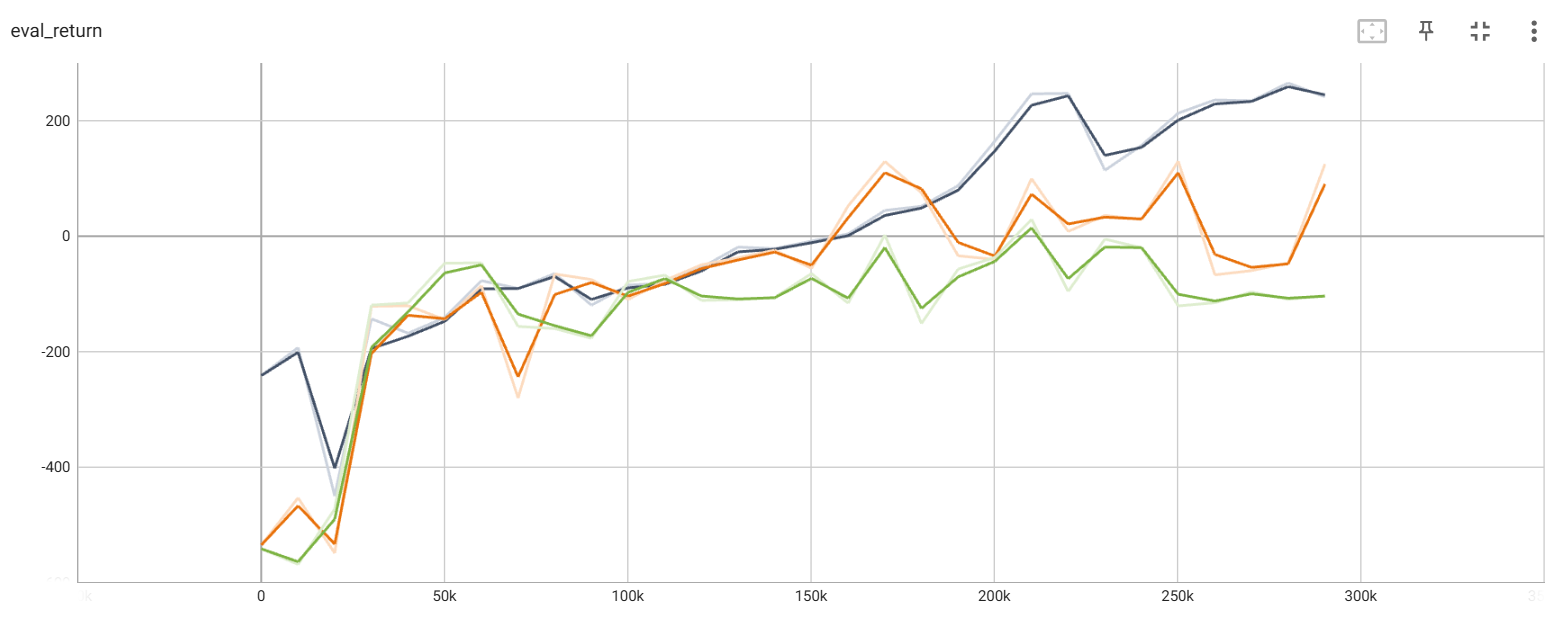
\includegraphics[width=0.8\textwidth]{imgs/dqn/lunarlander_doubleq.png}
    \caption{Lunar Lander DQN with Double Q-learning results}
    \label{fig:lunarlander_doubleq}
\end{figure}

\begin{figure}[H]
    \centering
    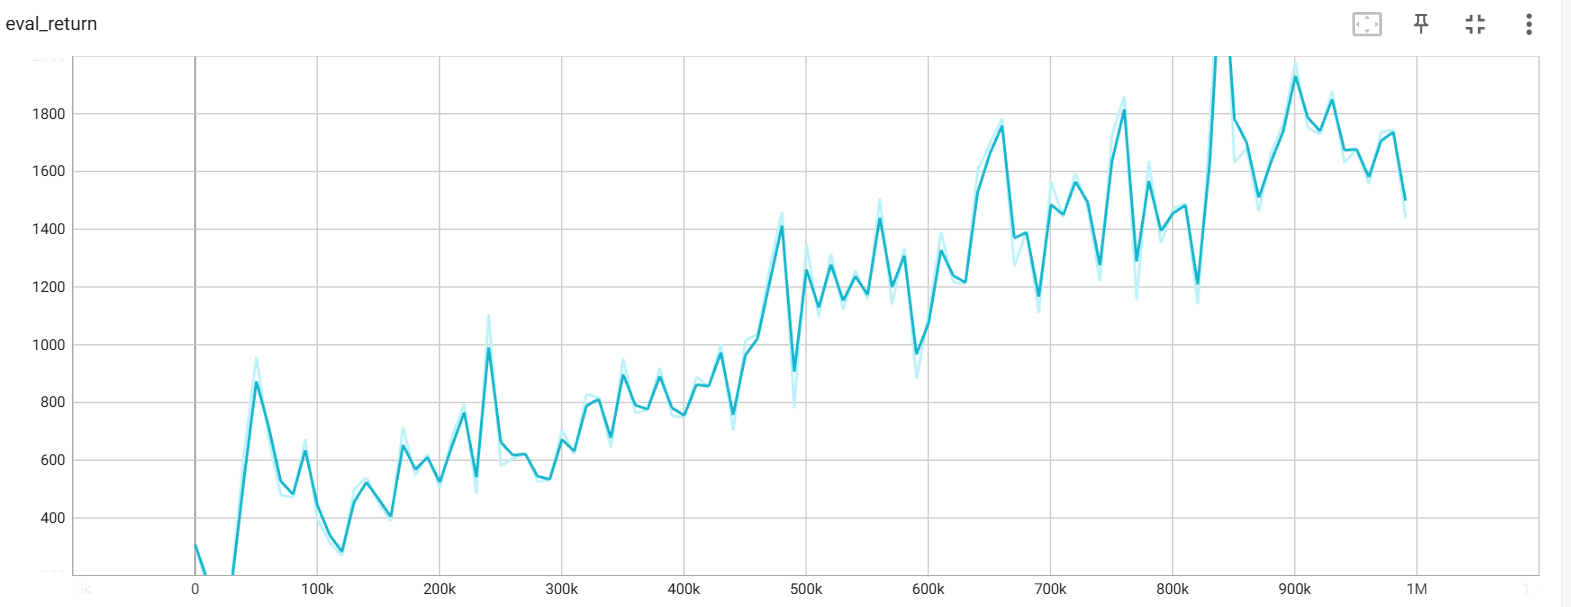
\includegraphics[width=0.8\textwidth]{imgs/dqn/mspacman.png}
    \caption{MsPacman DQN eval\_return results}
    \label{fig:mspacman}
\end{figure}

\begin{figure}[H]
    \centering
    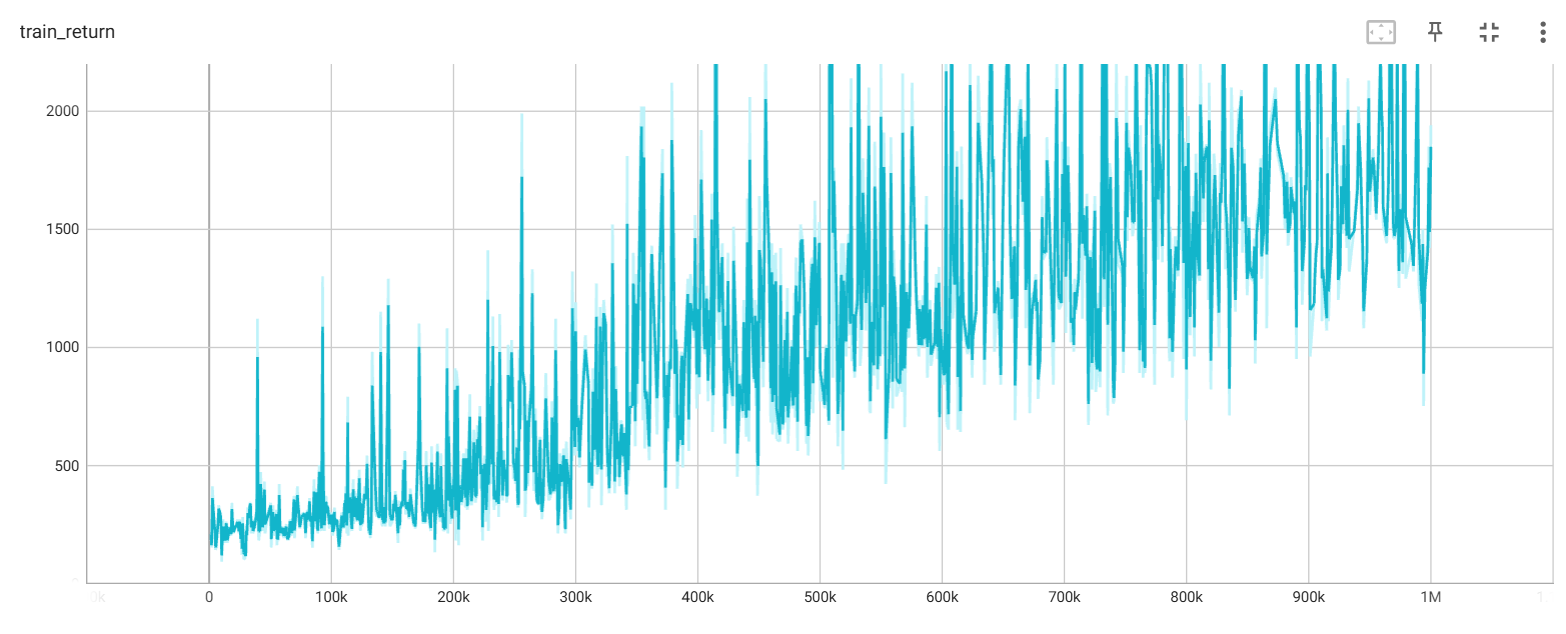
\includegraphics[width=0.8\textwidth]{imgs/dqn/mspacman_train_return.png}
    \caption{MsPacman DQN train\_return results}
    \label{fig:mspacman_train_return}
\end{figure}

\subsection{Experimenting with Hyperparameters} Now let's analyze the sensitivity of Q-learning to hyperparameters. Choose one hyperparameter of your choice and run at least three other settings of this hyperparameter, in addition to the one used in Question 1, and plot all four values on the same graph. Your choice what you experiment with, but you should explain why you chose this hyperparameter in the caption. Create four config files in \verb|experiments/dqn/hyperparameters|, and look in \verb|cs285/env_configs/basic_dqn_config.py| to see which hyperparameters you're able to change. You can use any of the base YAML files as a reference.

Hyperparameter options could include:
\begin{itemize}
    \item Learning rate
    \item Network architecture
    \item Exploration schedule (or, if you'd like, you can implement an alternative to $\epsilon$-greedy)
\end{itemize}